\documentclass[12pt]{article}

\setlength{\parindent}{4em}
\setlength{\parskip}{1em}
\usepackage{amsfonts}
\usepackage{amsmath}
\usepackage{graphicx}

\begin{document}

$\times  \div  \equiv  \neq  \ne  \geq  \ge  \leq  
\le  \not\le  \forall  \mid  \exists  \in  \not\in  \notin  \ni  \pi  
\theta  \alpha  \beta  \rightarrow  \Rightarrow$

%lines
\section{lines}

$\mid | \setminus \backslash$
\\
$$ A \backslash B = \{ a \in A \mid a \not\in B \} $$
$$ |x|^2 = x^2, |x| \geq 0 $$

%1cm
\section{1cm}

$$ \textrm{1cm(} x,y \textrm{) = the smallest positivte integer } z \textrm{ so that } x \mid z \textrm{ and } y \mid z$$

%dyadic
\section{dyadic}

$$the dyadic rationals are \left\{ \frac{a}{2^b} \middle|\: a,b integral \right\}\footnote{Hello World}$$ 

%verbatim
\section{verbatim}

If you type in \verb+ \verb| leading spaces|+ you get \verb|leading spaces.|
\begin{verbatim}
With verbatim you can get blank lines:
like ^that^ one.
\end{verbatim}

\clearpage

%mathfonts
\section{mathfonts}

$\mathfrak{hi}$
$\mathbb{hi}$
$\mathcal{hi}$

The permutation group $\mathfrak{G_n}$ is defined as 
$\{ \pi \in \mathbb{Z}^n \mid 1 \leq \pi \leq n$, all $\pi_i$
 distinct $\}$ and has cardinality $n!$, while the power set
 $\mathcal{P}(n)$ is defined as the family of all subsets of $S$, 
 and has cardinailty $2^{|S|}$.

 %territories

\begin{tabular}{lccr}
    \textbf{Name} & \textbf{Abbrv.} & \textbf{Capital} & \textbf{Population} \\
    \hline \\[1mm]
    Northwest Territories & NT & Yellowknife & 41 462 \\
    Nunavut & NU & Iqualuit & 31 906 \\
    Yukon & YT & Whitehorse & 33897 \\
\end{tabular}

 %reals

$$
\begin{array}{lll}
    \pi & 3.14159 & 4\sum_{4\geq 1}(-1)^{k+1}/(2k-1) \\
    \pi & 1.61803 & (1 + \sqrt{5})/2 \\
    e & 2.71828 & \sum_{k\geq 0} 1/(k!) \\
\end{array}
$$

 %Llinealg

$$
 \begin{vmatrix}
    a & b & c \\
    d & e & f\\
    g & h & i\\
 \end{vmatrix}
 = det 
 \begin{bmatrix}
    a & b & c \\
    d & e & f\\
    g & h & i\\
 \end{bmatrix}
$$

%1000 words

\clearpage
\begin{figure}[b]
    \centering
    
    Woah! A house
    \begin{center}
        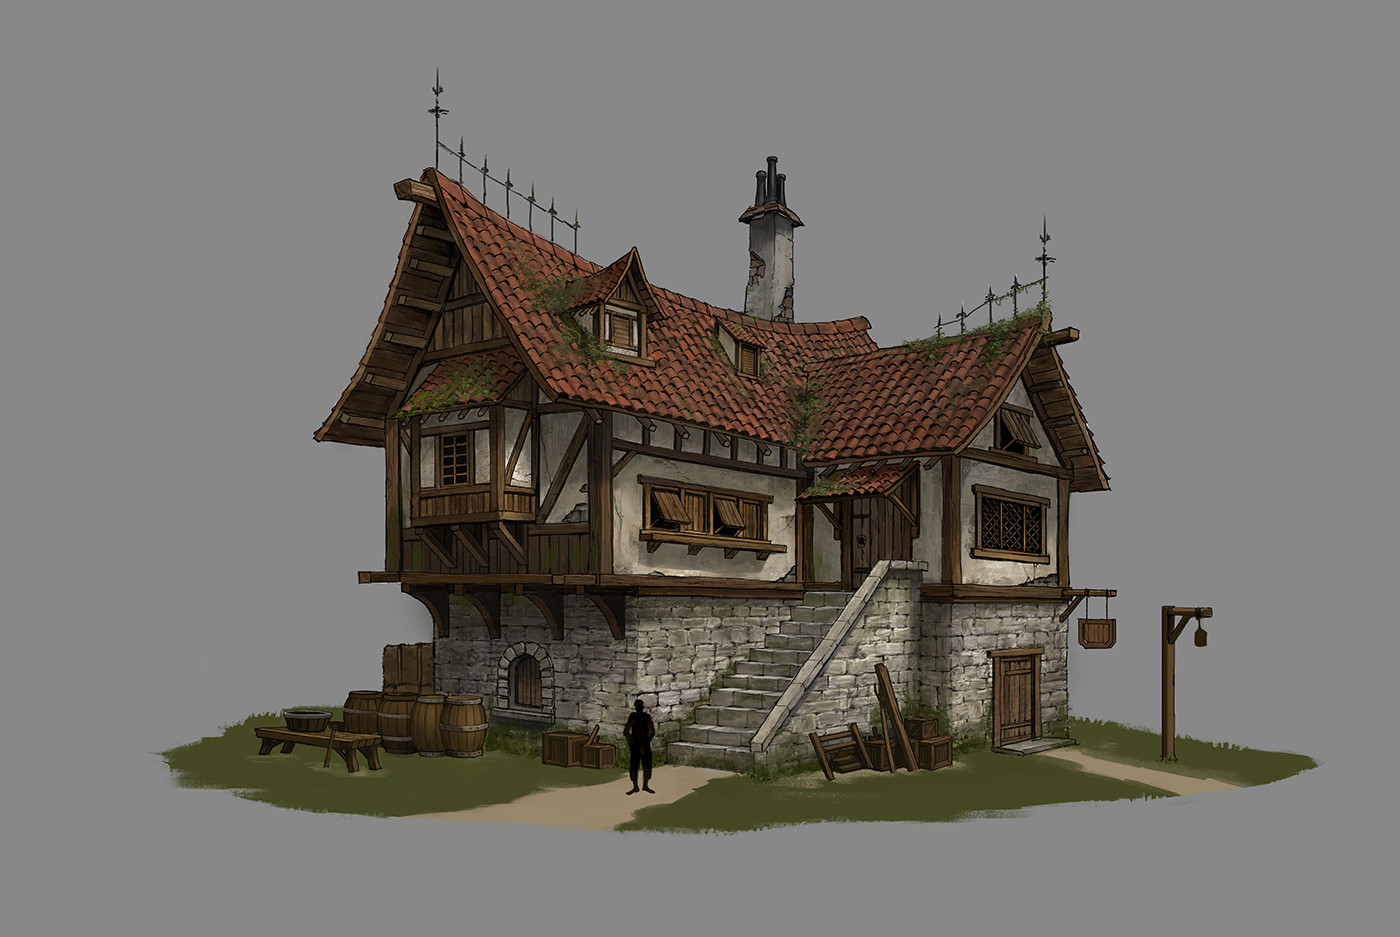
\includegraphics[scale = 1]{donghee-han-d2.jpg}
    \end{center}
    \caption{A medieval style of house}
    
\end{figure}

\clearpage
\begin{tabular}{lcr}
    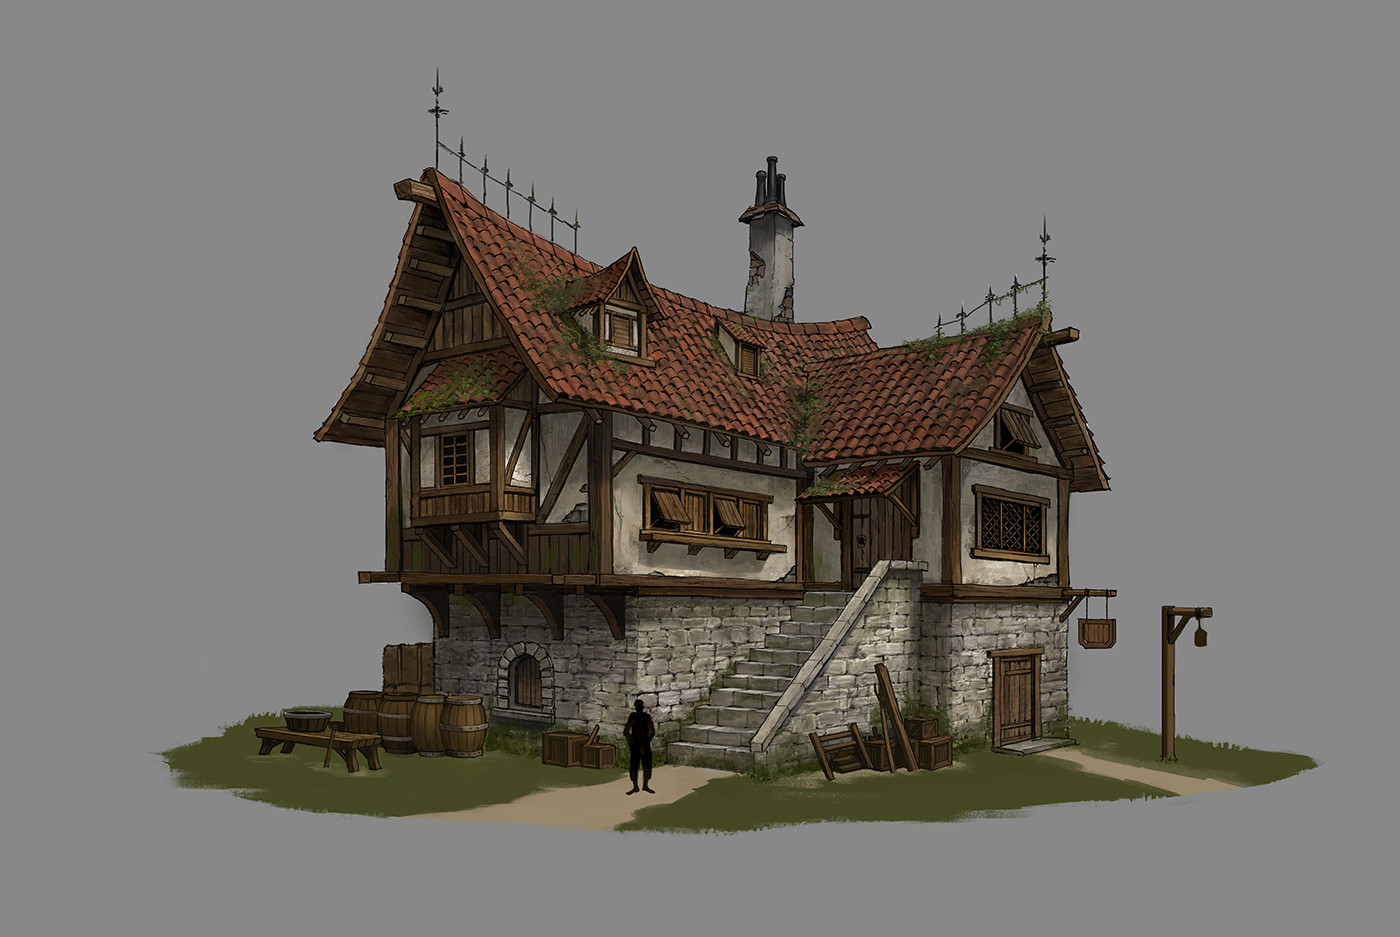
\includegraphics[scale = 0.3]{donghee-han-d2.jpg} & 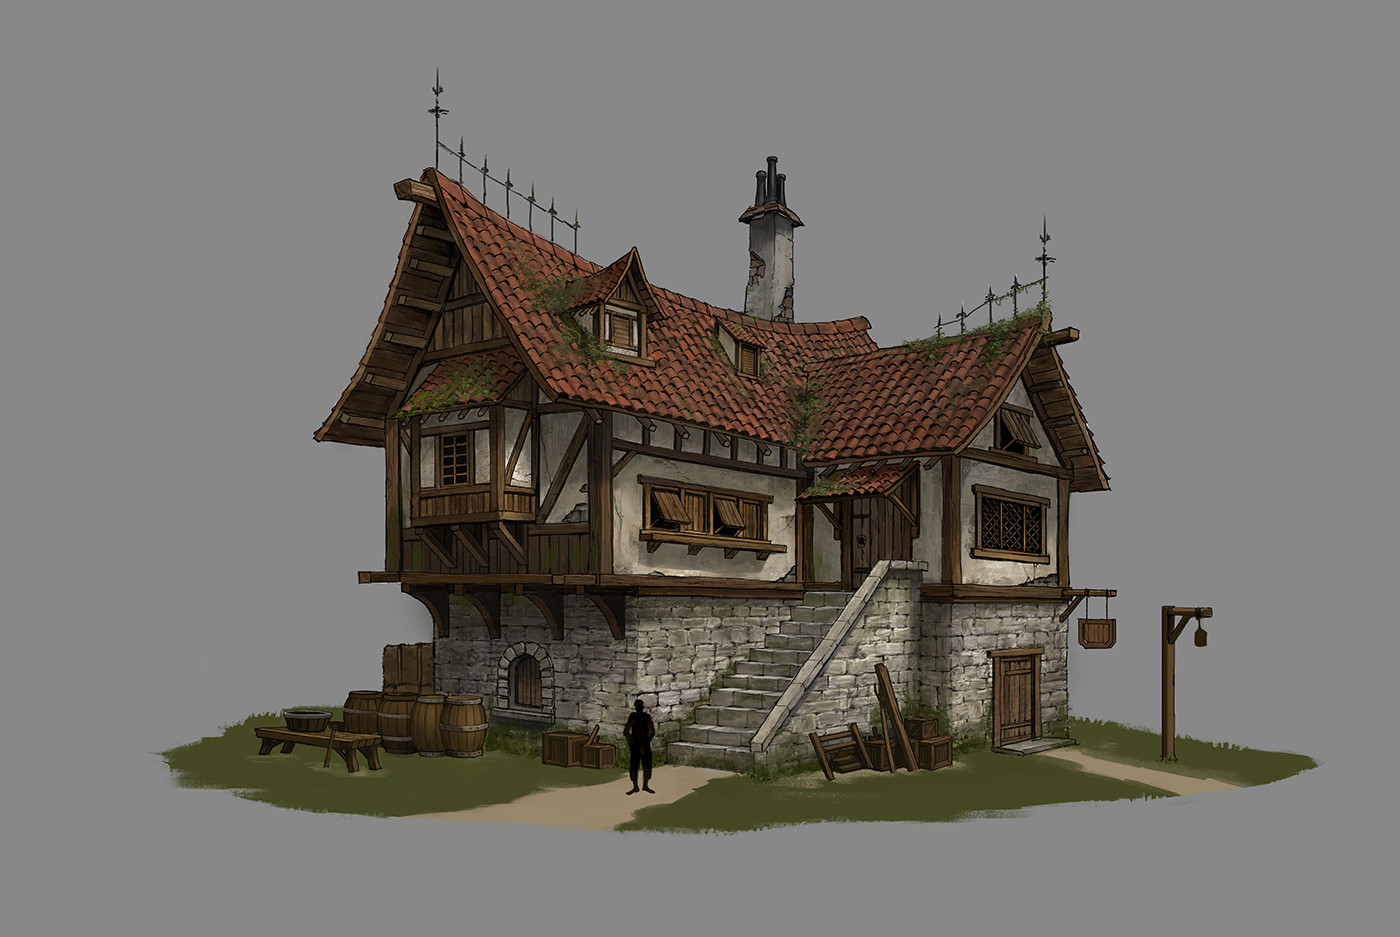
\includegraphics[scale = 0.3]{donghee-han-d2.jpg} & 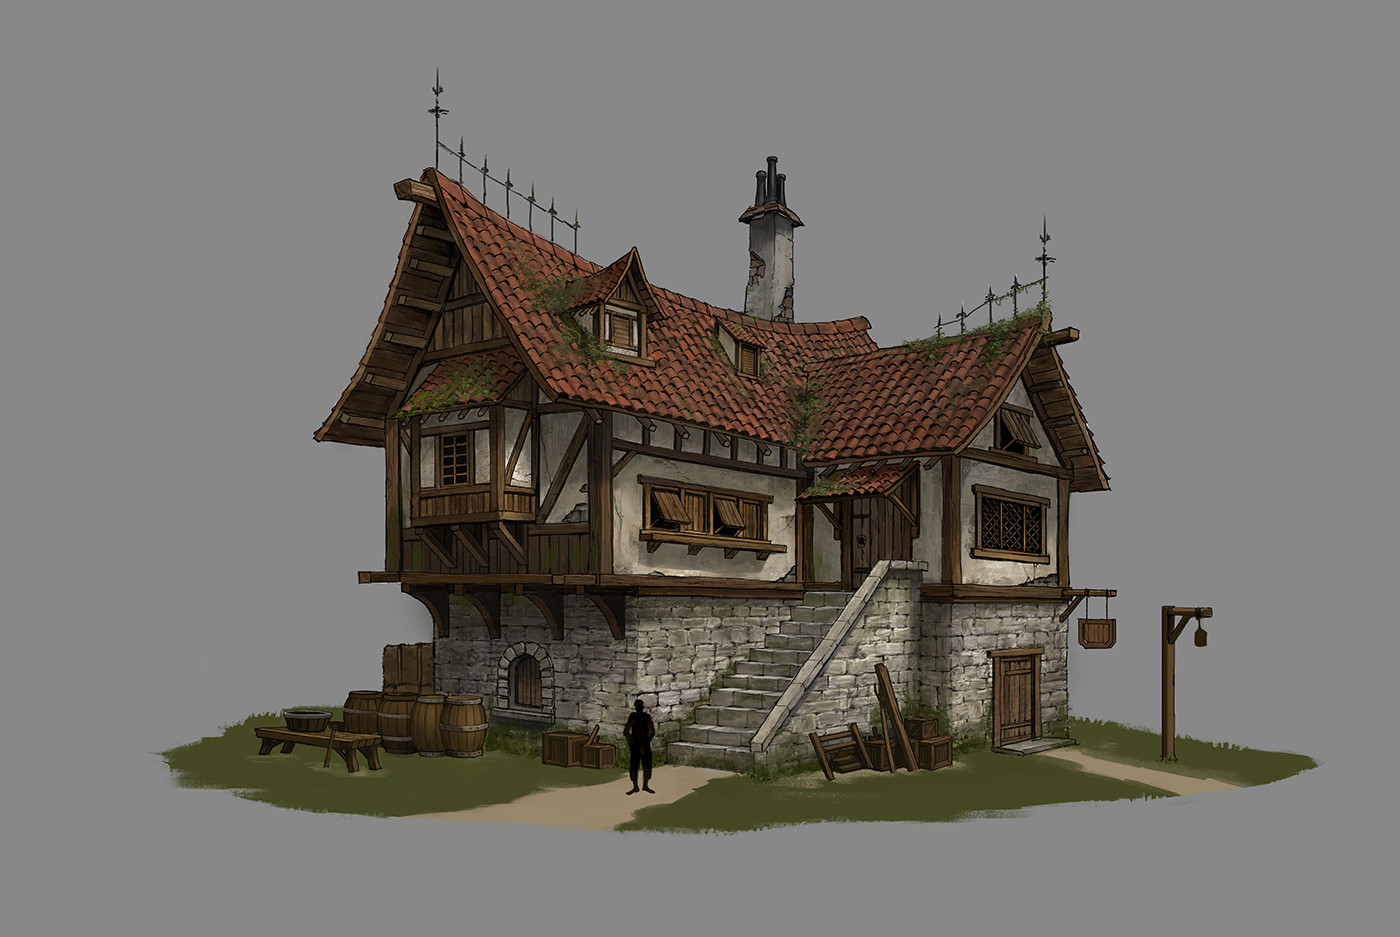
\includegraphics[scale = 0.3]{donghee-han-d2.jpg} \\[0.4cm]
    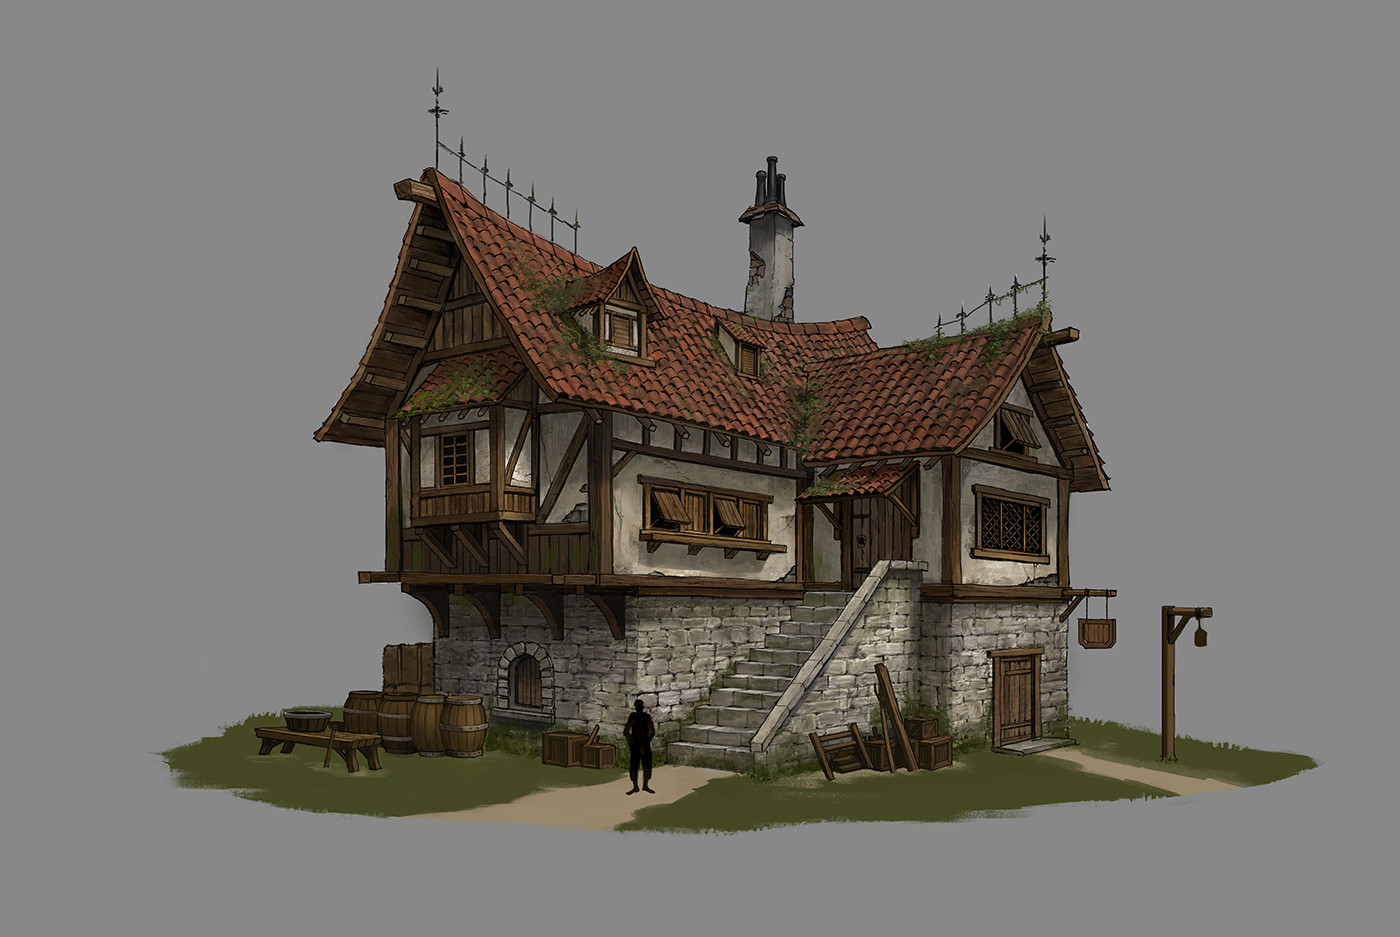
\includegraphics[scale = 0.3]{donghee-han-d2.jpg} & 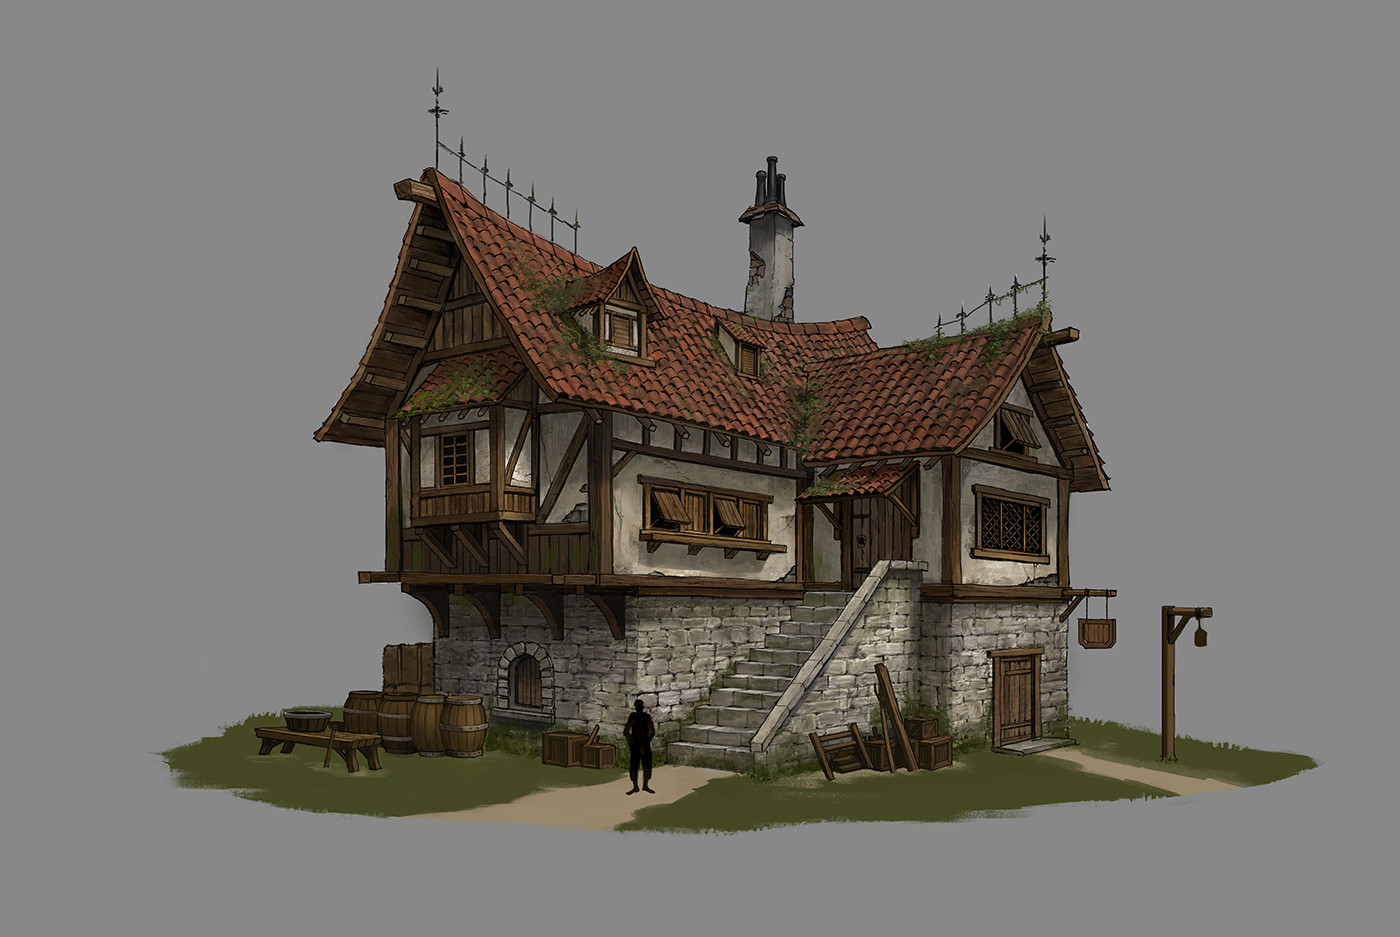
\includegraphics[scale = 0.3]{donghee-han-d2.jpg} & 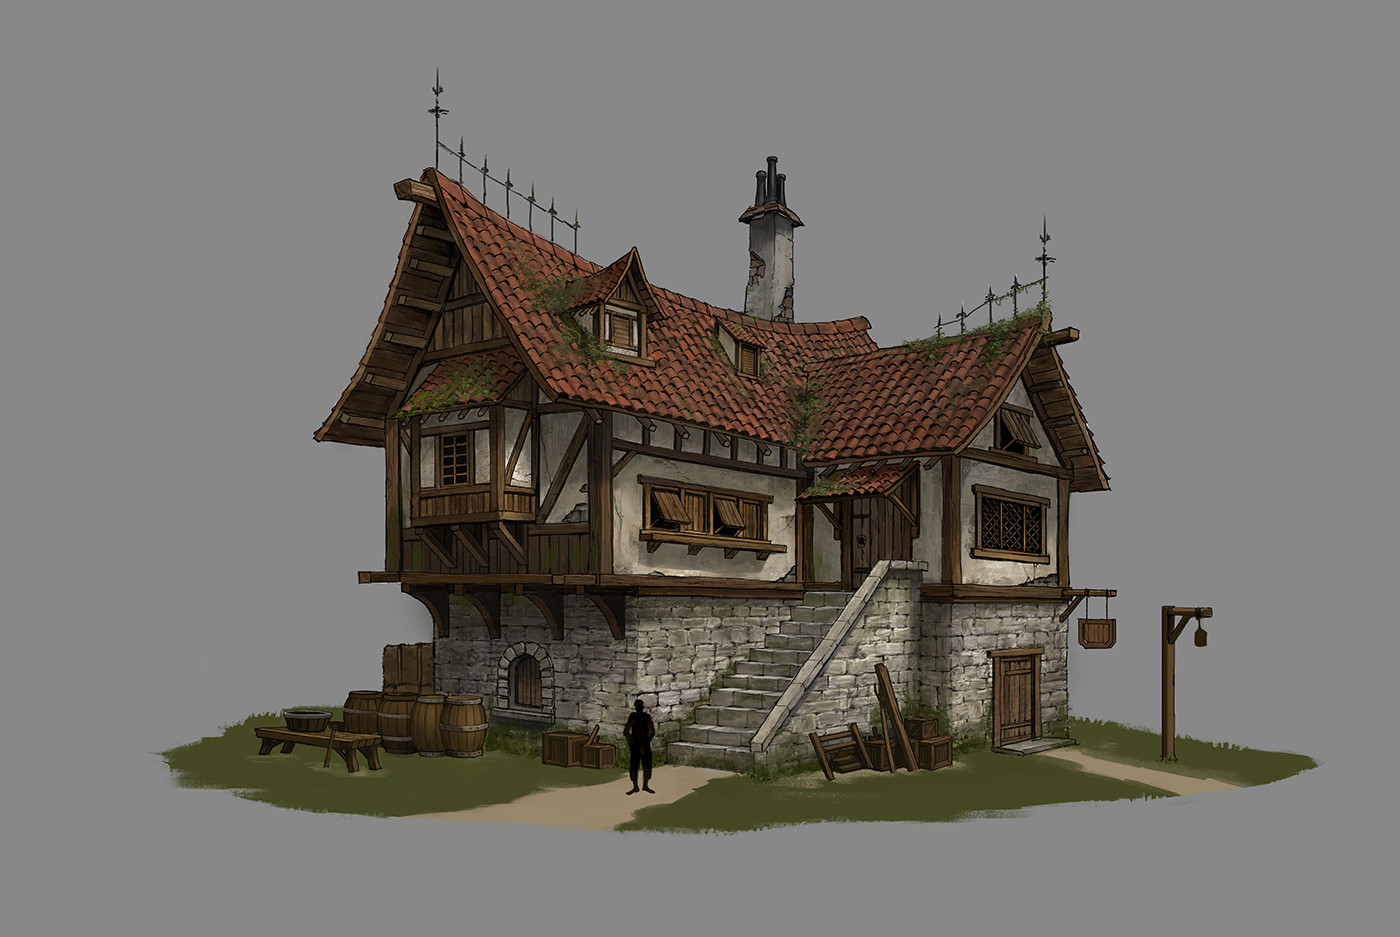
\includegraphics[scale = 0.3]{donghee-han-d2.jpg} \\[0.4cm]
    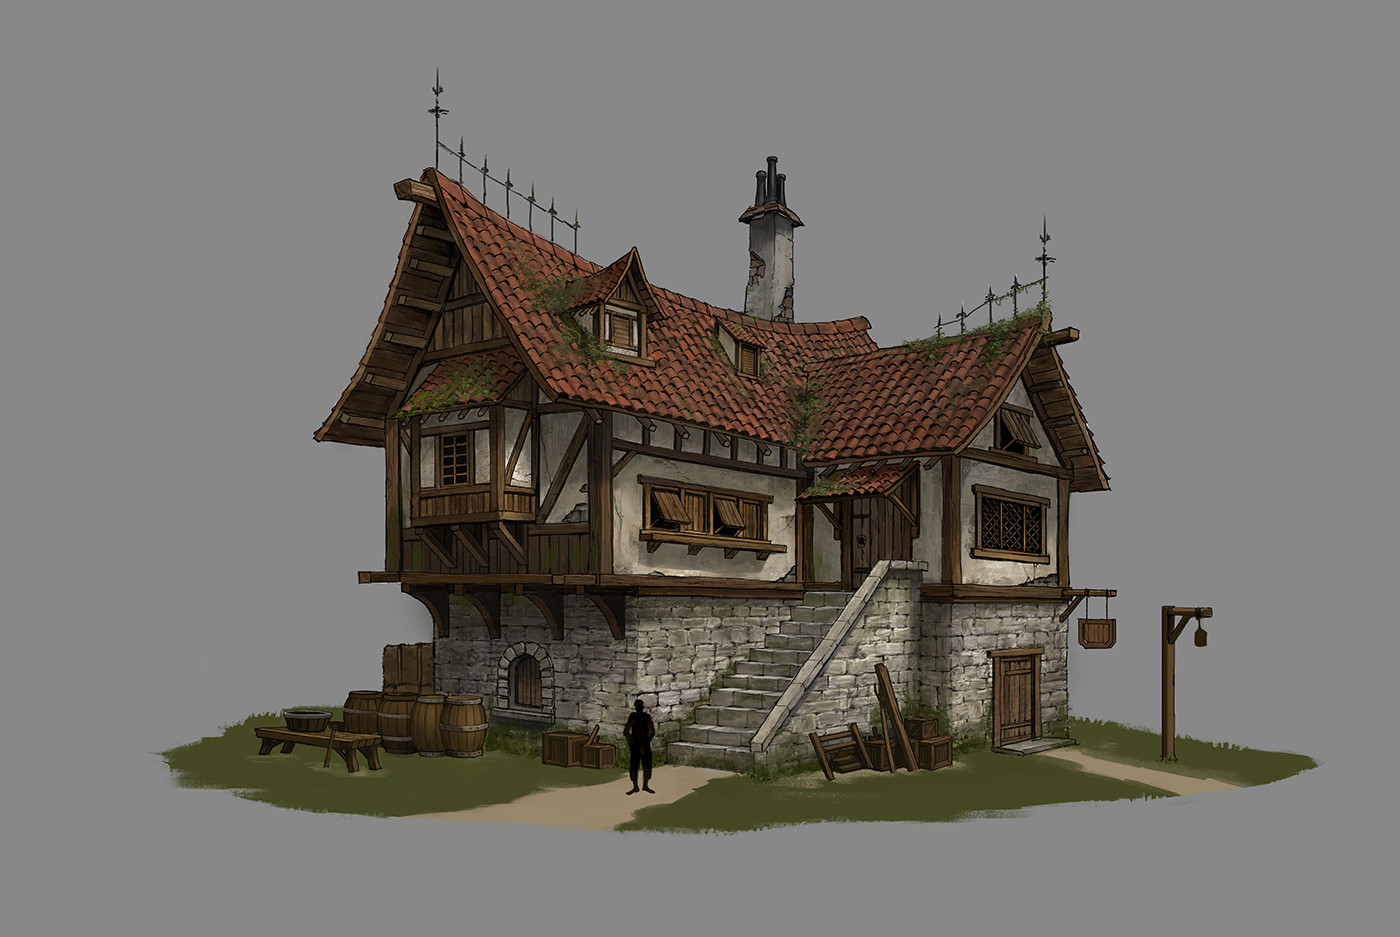
\includegraphics[scale = 0.3]{donghee-han-d2.jpg} & 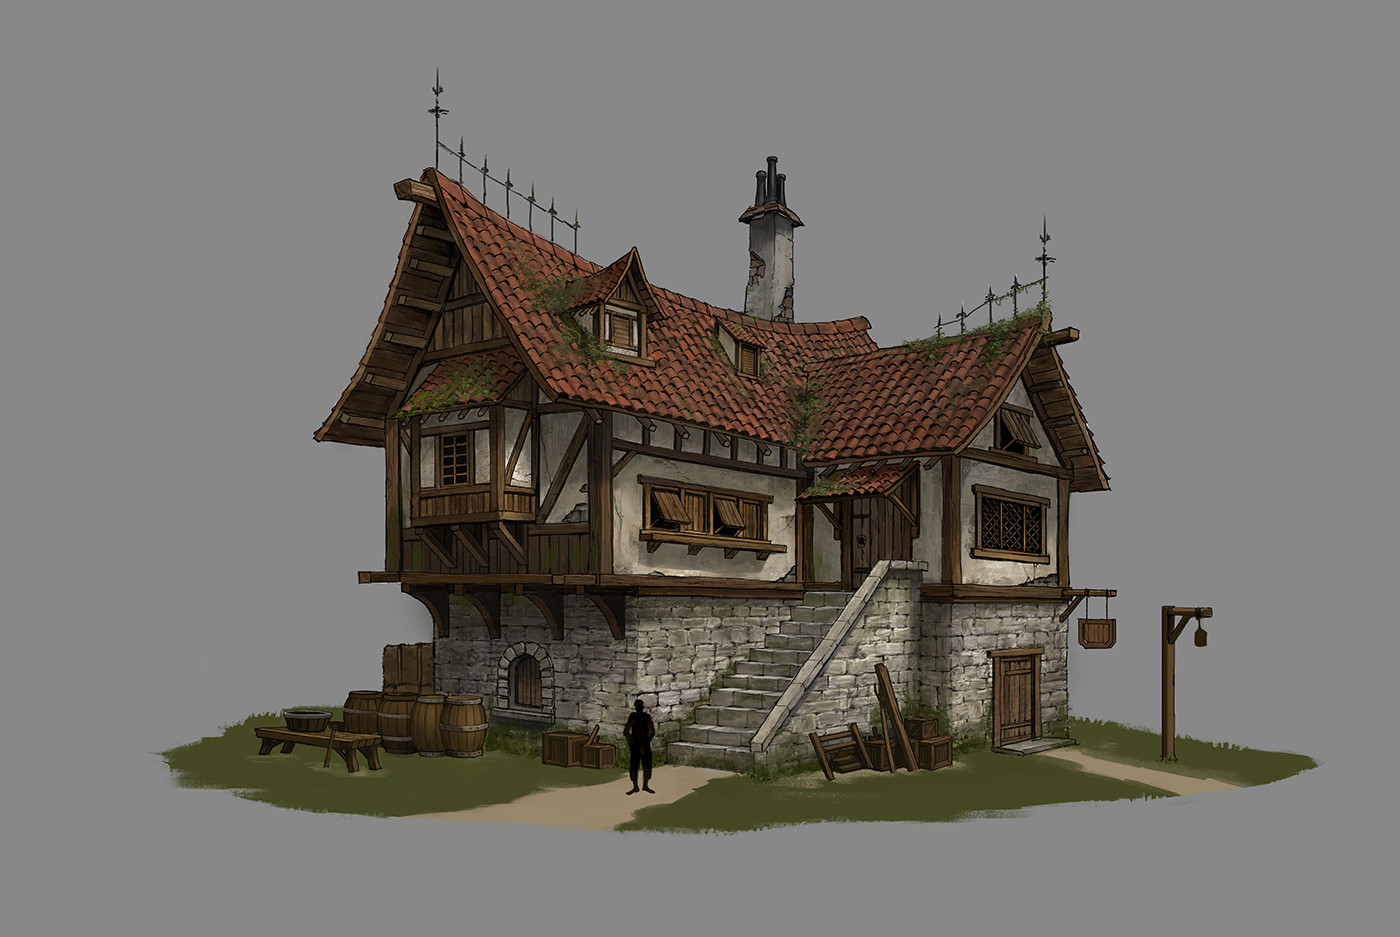
\includegraphics[scale = 0.3]{donghee-han-d2.jpg} & 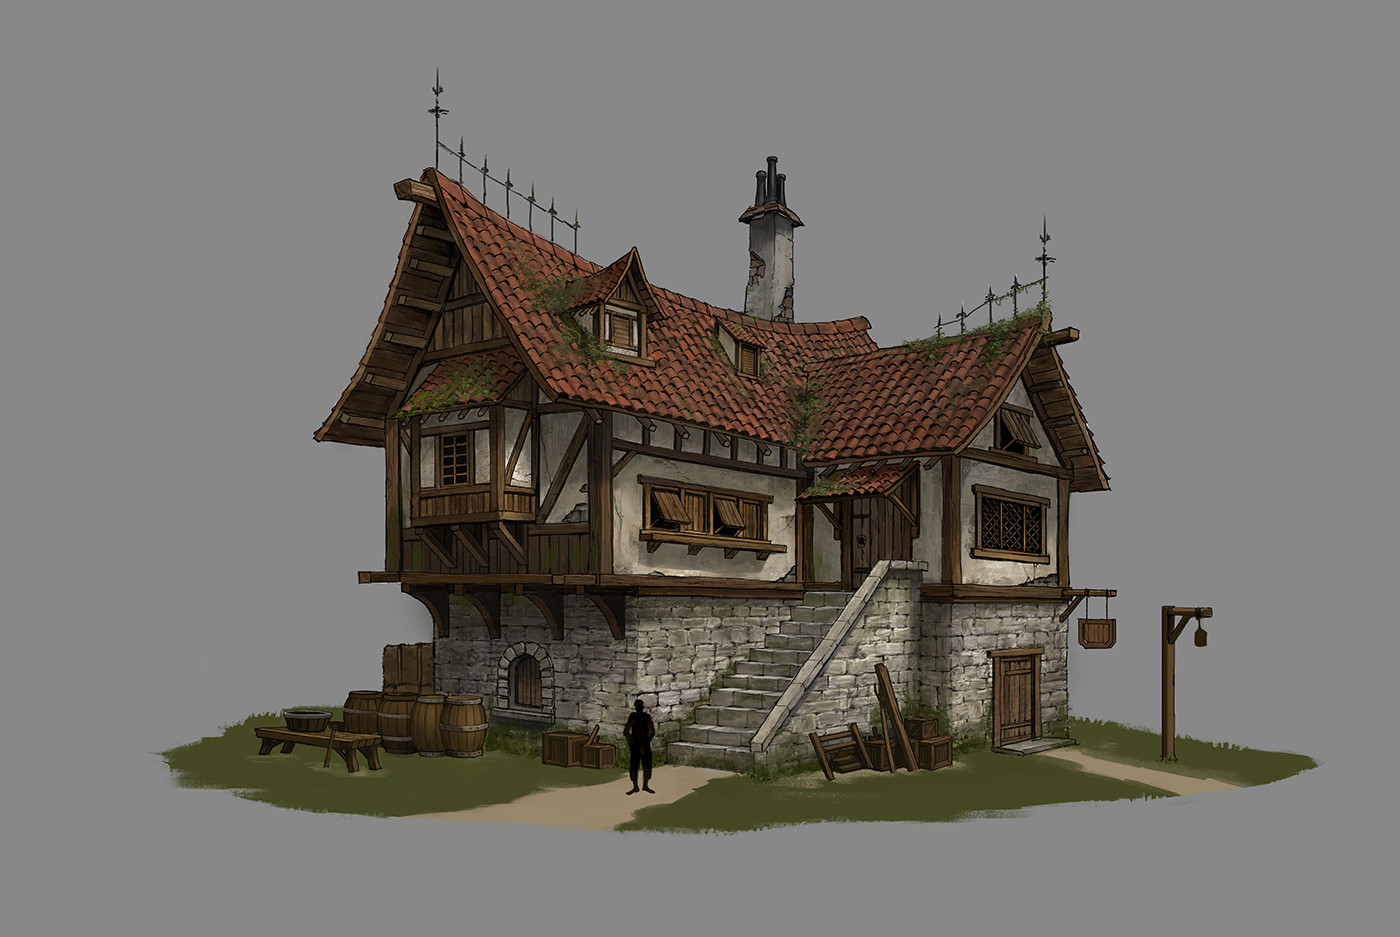
\includegraphics[scale = 0.3]{donghee-han-d2.jpg} \\[0.4cm]
\end{tabular}

%bodyparts
\appendix

\section{appendix}



\end{document}